\documentclass[12pt]{report}

% PACKAGE USING
\usepackage[top = 1in, bottom = 1in, left = 0.75in, right = 0.75in]{geometry}
\usepackage{amsmath}
\usepackage{xcolor}
\usepackage{graphicx}
\usepackage{url, hyperref}
\hypersetup{
    colorlinks = true,
    urlcolor = blue,
    citecolor = red
}


\begin{document}

\begin{titlepage}
    \begin{center}
        \vspace*{5cm}
 
        \Huge{\textbf{Commodity Report Assignment}}
 
        \vspace{0.5cm}
        \LARGE{Natural Whitish Sesame Seeds}\\
        \Large{and}\\
        \LARGE{Sugar}
             
        \vspace{1.5cm}
 
        \large{\textbf{Subhrajyoty Roy}}\\
        \large{\textbf{MB1911}}
 
        \vspace{2cm}
             
        \textit{Assignment for Quantitative Finance course\\
        as a part of Master of Statistics curriculum}\\
        \vspace{0.5cm}
        \textbf{Session: } 2020-21\\
        Indian Statistical Institute, Kolkata

        \vfill
        
        \begin{flushright}
            \normalsize{\today}            
        \end{flushright}
    \end{center}
\end{titlepage}

\tableofcontents
\pagebreak


\part{Sesame Seeds}
\setcounter{chapter}{1}

\section{Introduction}

% ABOUT SEASAME
Sesame (\textit{Sesamum Indicum}) is a flowering plant of the genus Sesamum comprising of about $20$ other species of variants of Sesame seeds. It is one of the oldest oilseed crops known, domesticated well over $3000$ years ago, possibly due to its sturdy capabilities of withstanding harsh conditions of barren land, where most of the other crops fail. It is also a robust crop that needs little farming support, can be grown in drought conditions, in high heat, with residual moisture in soil after monsoons are gone, or even when rains fail or when rains are excessive. Also, sesame seeds are one of the oilseeds with the highest oil contents, thus giving another incentive for the subsistence farmers to grow the crop. 

Sesame seeds are a common ingredient in different cuisines across the world due to its rich, nutty flavor, as well as its medicinal values to facilitate digestion and reduce hypertension. This growing popularity of sesame seeds as a functional ingredient in several foods is a key demand driving factor in the market.  Furthermore, the increasing application of the product as an anti-oxidant in various pharmaceutical formulations is expected to further drive the growth of the Indian market in the future. Also, because of its high yield and better weather tolerance, various companies are focusing on sesame-based prepared (or packeted) foods, thus expanding both the international and domestic market further.


\section{Overview of the Market}


\begin{figure}[h]
    \centering
    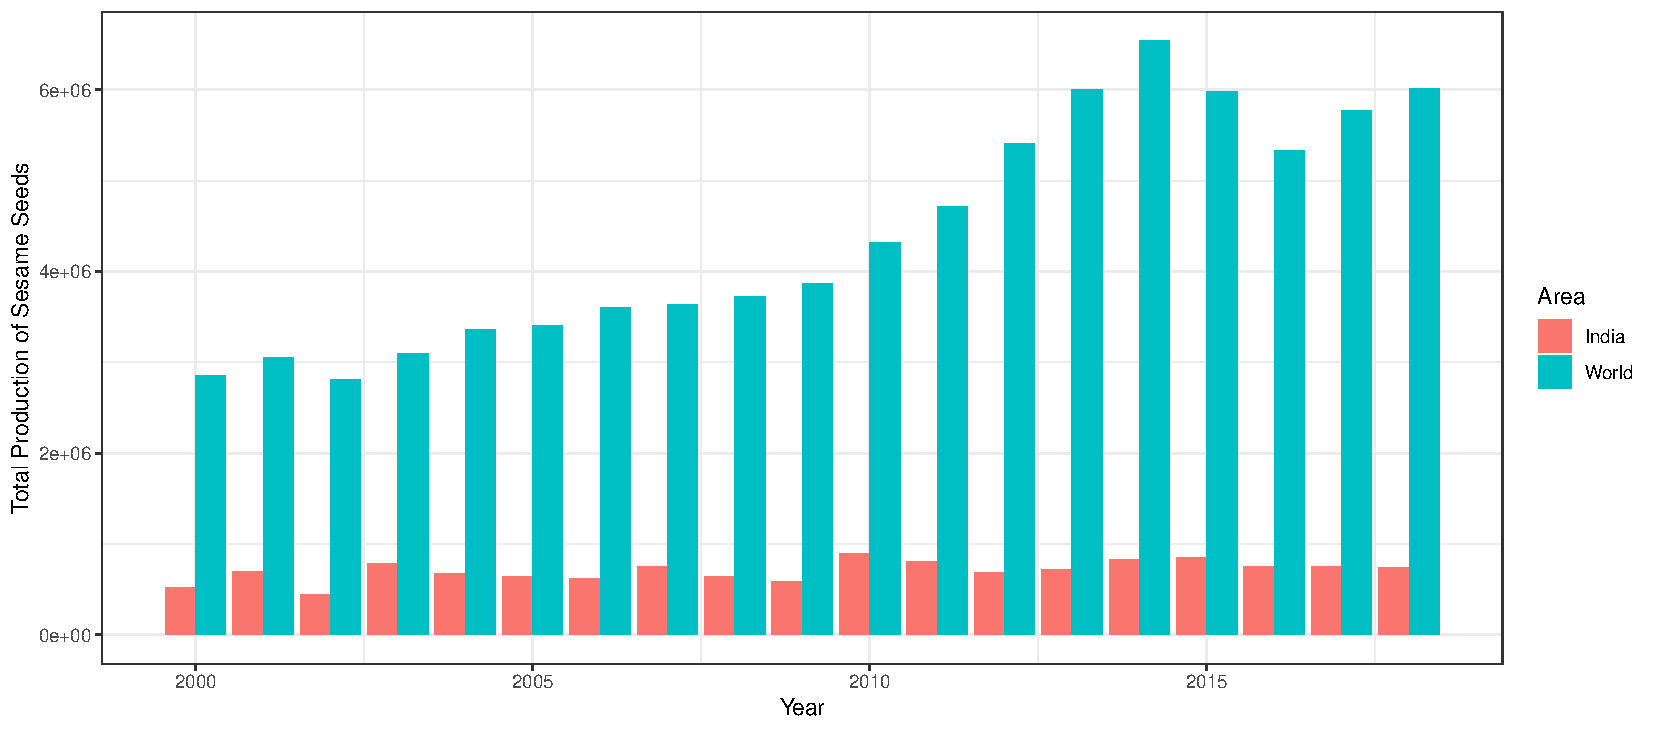
\includegraphics[width = 0.8\linewidth]{sesame-total.pdf}
    \caption{Yearly total production of sesame seeds in India and in the World}
    \label{fig:sesame-total}
\end{figure}


After Tanzania and Mayanmar, India is the 3rd largest producer of Seasame seeds~\cite{FAO-site}. In 2018, India produced a whooping $7.46$ metric tonnes of sesame seeds, while the global production was $63.6$ metric tonnes. While the absolute production of sesame seeds remained constant over the last $5$ years, as shown in Figure~\ref{fig:sesame-total}, the contribution of India to global production declined due to rapidly increasing production rates in the Middle East and North African countries due to their desert-like conditions suitable for the growth of sesame seeds. Currently, India shares a top position on the leaderboard for the global contribution of $11.7\%$ with several other major producers like Tanzania, Myanmar, Sudan, Nigeria, China, Ethiopia, South Sudan, Burkina Faso, Chad, Uganda, etc. An upward trend is manifested for future productions; the global sesame market is anticipated to expand to 9.5 million tonnes by 2025.

In the context of India, sesame cultivation spread across all parts of the country except in the northern and north-eastern regions. Most of the production is concentrated in central and southern parts of the country including Madhya Pradesh, Uttar Pradesh, Andhra Pradesh, Rajasthan, Gujarat, Maharashtra, Orissa, Karnataka, and Tamil Nadu. Collectively, these states produce more than $83\%$ of the total sesame production in India. Although sesame seeds can be grown in all three seasons throughout the year, the majority of the production of sesame seeds in India is based on monsoon seasons (generally from May-June to December-January) as a part of rainfed Kharif crops~\cite{ncdex}.

According to data from the Agricultural Ministry of India~\cite{agro-ministry, eco-times}, the export of sesame seeds during April 2019-March 2020 was 2,82,236 tonnes, valued at Rs 3,723 crore and the average market size of sesame in India in the last five years has been Rs 7,280 crore.


\begin{figure}[h]
    \centering
    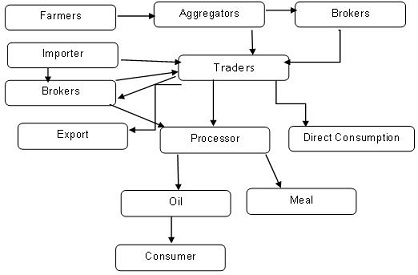
\includegraphics[width = 0.8\linewidth]{SesameSeeds_Value_Chain.jpg}
    \caption{Value chain of Sesame seeds}
    \label{fig:sesame-vc}
\end{figure}

The value chain from farmers to the consumers for sesame seeds is quite convoluted (Figure~\ref{fig:sesame-vc}). There remain various aggregators, brokers, and traders who work as the intermediary between farmers and the trade markets. These traders usually process the seeds to brew oil and different food (or spice) byproducts, which are finally sold to the consumer.


\section{Financial Contracts}

The first financial contract on Natural Whitish Sesame Seeds (SESAMESEED) was launched on March 30, 2005, by National Commodity Derivatives \& Exchange Ltd. (NCDEX)~\cite{ncdex-circular1}. The initial contracts were FUTCOM (Futures contract on Commodity) for 3-5 months. Upon expiry of these contracts, both buyers and sellers are obliged to meet the respective demand or supply of sesame seeds by physical delivery through the basis centre of the exchange NCDEX at Rajkot, India. The contracts also specify the quality of the delivery in terms of a mixture of whitish sesame seeds with other colour seeds. Since there remains uncertainty in meeting the exact quality requirements, different quality specifications of admixture are allowed to be delivered subject to different premium / discounted strike prices, as specified by the contract terms. 

While these future contracts remained popular during 2005-2006, the volume of such trades consistently declined in the first quarter of 2007, and NCDEX closed the futures on sesame seeds. With the recent surge in demand in the European market and its consistently increasing potential in recent times, NCDEX relaunched Natural Whitish Sesame Seeds (SESAMESEED) Futures from August 26, 2020, again with 3 types of expiry dates in October, November and December, 2020~\cite{ncdex-circular2, eco-times}. NCDEX speculates that Natural Whitish Sesame Seeds futures can be an effective hedging instrument for all the stakeholders for efficient price discovery and risk management, as well as introduce new business opportunities for farmers and value chain participants (VCPs).

The new future contracts come with more regulations and specifications than its former counterpart. For example, whereas the buyer of the underlying is not allowed to default (In case of defaults, the clearing corporation holds the right to sell goods on account of buyers to recover any dues), the seller is allowed to default to meet the obligations at the cost of a penalty price, due to the uncertain nature of supply of agricultural commodities. The total amount of penalty is calculated as $3\%$ of the settlement price added to a replacement cost (with highest spot prices). In these futures contracts, all open positions are settled daily based on the Daily Settlement Price (DSP) that is disseminated by the Exchange at the end of every trading day. Average daily turnovers (ADTV) from these futures are currently Rs. 7.74 lakhs, with a volume totalling Rs. 53.16 lakhs in August 2020 and Rs. 48.10 lakhs in September 2020. 
 

\section{Pricing Model}
\label{sec:price-sesame}

There are several factors that should be accounted for in the pricing model approaches for the sesameseed futures.

\begin{enumerate}
    \item Prices of the other competitive oils in India like soy oil, mustard oil, etc.
    \item International price movement of sesame seeds at Ethiopia Commodity Exchange, which is the largest exchange traded market for sesame seeds.
    \item Celebrations and festival seasons when these seeds are consumed in larger quantities. Hence, a seasonal effect has to be introduced in the modelling approach.
\end{enumerate}


The pricing of these futures can be determined by considering two equivalent strategies. In the first strategy, the person buys a future at price $P$ with obligations to buy the underlying at a strike price $K$ in future. For this, he/she holds the future contract and invest $K/\prod_{t = 1}^T (1 + r_t)$ in the bank with interest rates $r_t$ at time period $t$, and with expiry date $T$. Another strategy would be to hold onto the underlying asset at present until the expiry. Since, both of these pays $S_T$, the price of the underlying at expiry, by use of law of one price we must have $P + K/\prod_{t = 1}^T (1 + r_t) = S_0$, where $S_0$ is the current spot price of the underlying at the time of issuing the future contract. Hence, the price of the future can be determined as;

$$
P = S_0 - \frac{K}{\prod_{t = 1}^T (1 + r_t)}
$$

However, National Commodity Clearing Limited (NCCL) uses a risk based margin model that generates an initial margin requirements specific to each contract, and expected to compensate at least $99\%$ VaR (Value at Risk) and Margin Period of Risk (MPOR) will be $3$ days. In case of unidirectional price movements and increased volatility, an additional special margin may be imposed by the exchange on either the seller or buyer side or both.




\part{Sugar}
\setcounter{chapter}{2}
\setcounter{section}{0}

\section{Introduction}

There are two primary sugar-producing crops, namely Sugar cane (\textit{Saccharum officinarum}) and Sugar beets (\textit{Beta vulgaris})~\cite{fao-sugar-def}. While canes are responsible for about $75\%$ of global sugar production, beets contribute about $20\%$, and the rest $5\%$ are produced from the sap of certain species of maple trees, from sweet sorghum when cultivated explicitly for making syrup and from sugar palm. Despite being a commodity for mass consumption and the cheapest source of energy, sugar is generally viewed as a cash crop and also as a livestock fodder to some extent~\cite{wiki-sugar}. As a source of food, sugar cane is used for various products like crystalized sugar, sugar cane juice, syrups, molasses, juggery, candies and various alcoholic and non-alcoholic beverages.

Various biofuels like ethanol are generally available as a byproduct of sugar production. Brazil has turned this opportunity into the substitute of gasoline as a widely used fuel in the cars. It is speculated that ethanol may become the primary product of sugarcane processing, rather than sugar in Brazil. Sugarcane bagasse is another potentially abundant source of energy for large producers of sugarcane, such as Brazil, India and China. With the use of the latest technologies, bagasse produced annually in Brazil has the potential of meeting $20\%$ of Brazil's energy consumption by 2020~\cite{brazil-article}.

Depending upon the variety and sowing time it takes about 12 to 18 months to mature. While generally, the start of a year is the period of planting and year-end is the period of harvesting, in some states of India, sugar cane is grown around the year. sugar comes in three forms: Large crystals (L-grade), Medium crystals (M-grade) and Small crystals (S grade). M and S grades form about $80\%$ of total sugar production and are usually used for trading in exchanges.


\section{Overview of the Market}

\begin{figure}[h]
    \centering
    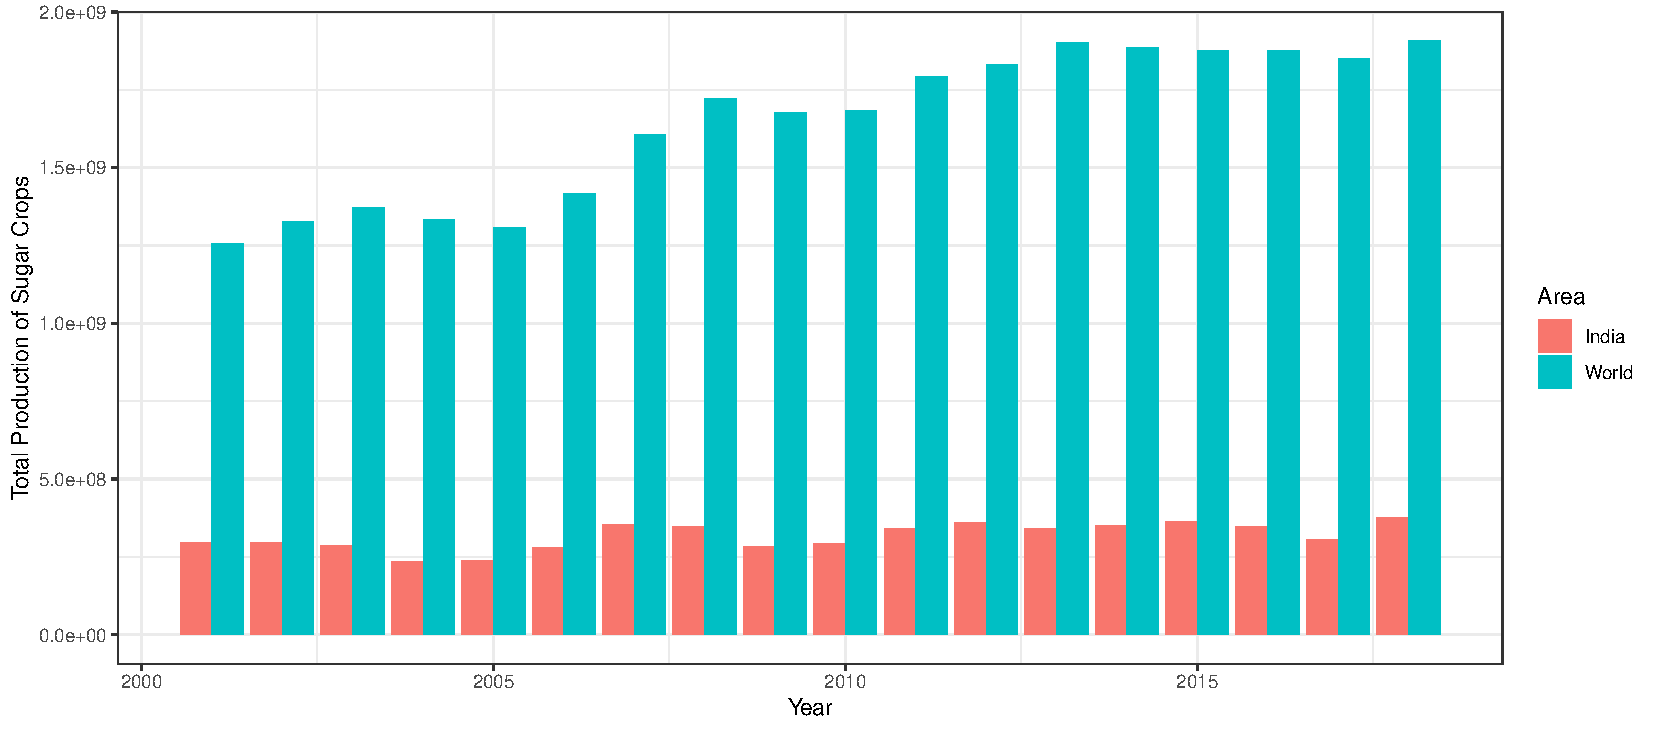
\includegraphics[width = 0.8\linewidth]{sugar-total.pdf}
    \caption{Yearly total production of sugar cane in India and in the World}
    \label{fig:sugar-total}
\end{figure}

The production of sugar in India comes only from sugar canes, but not from sugar beets which are primarily dominated by the US, Turkey, Ukraine, Poland and Russia. However, the global production of sugarcane about $1.9$ billion tonnes, with India contributing about $20\%$ of the global production standing 2nd in the leaderboard behind Brazil. While the global production of sugarcane has been rising considerably for last $20$ years as shown in Figure~\ref{fig:sugar-total}, the production of India remained at about the same level similar to the scenario with sesame seeds. However, India is also the largest consumer of sugar in the world with demand nearly equaling the supply in most cases, thus, having only a minimal international supply of the sugar crops.

In the context of India, Maharashtra is the largest producer of sugar in the country followed by Uttar Pradesh. Together these two states account for over $60\%$ of the total sugar production in the country. Since sugar production is effected by acreage and yield, sugarcane availability, recovery percentage and duration of crushing, various states majors in each of these factors. Of these, the area is highest in Uttar Pradesh followed by Maharashtra, the yield is highest in Tamil Nadu, and average recovery is highest in Maharashtra. The average duration of crushing is almost equal in Maharashtra, Gujarat and Tamil Nadu (about 150 days). 


\begin{figure}[h]
    \centering
    
\includegraphics[width = 0.8\linewidth]{sugar_value_chain.jpg}
    \caption{Value chain for Sugar cane in India}
    \label{fig:sugar-vc}
\end{figure}


Unlike sesame seeds, the value chain for sugar cane in India is very simple (Figure~\ref{fig:sugar-vc}), possibly due to an insignificant amount of international supply. After the harvest of sugar cane by the farmers, they are processed in sugar mills and various byproducts are sold to agents and brokers. These brokers trade in the exchanges to sell the sugar products to the retailer, who ultimately sells it to the consumers.


\section{Financial Contracts}

For sugar cane, NCDEX started with only one future contracts introduced on July 27, 2004, with contracts with expiry dates at October 2004, November 2004, December 2004 and April 2005, for Sugar M (medium size sugar crystals). The trading unit and delivery unit was 10 MT and tick size of Rs. $1$ with Kolhapur as the basis centre. With the considerable rise in the volume of trading, on 9th June 2005, NCDEX launched future contracts SUGARM200 and SUGARS150, for sugar M and sugar S grade with units of 200 MT and 150 MT, with the addition of Kolkata as a delivery centre. From then several other modifications of these contracts have been done, with the addition of other delivery centres - Belgaum, Delhi, Pune, Sangli and Solapur etc. The latest modification was the removal of the direct delivery of the underlying upon expiry of the contracts, allowing only trackable delivery via the exchange. All of these future contracts specify the quality of the sugar gauged in ICUMSA number, which assesses the chemical properties of sugar for grading.  

In the 2009-10 seasons, sugar production fell to 18.9 million tonnes, causing a sudden jump in the prices, obliging NCDEX to temporarily close the trading of contracts. Average open interest before delisting of sugar contracts was close to $125000$ with an average daily trading volume of about $50,000$ MT. After relisting on December 27, 2011, even with several Govt. regulations, the number of traded contracts boomed and showed an increment in traded volumes, rising from a daily traded volume from $20,000$ tonnes to $50,000$ tonnes.  Sugar contract is a high delivery contract with very fewer defaults, which suggests interest of cash and carry arbitrage as well. After the announcement of the removal of sugar stock limit on 22nd November, open interest and trading volume have increased drastically in NCDEX.


\section{Pricing Model}

There are several factors that should be accounted for in the pricing model approaches for these futures.

\begin{enumerate}
    \item The Central Government fixes the Fair and Remunerative Price (FRP) for sugarcane. Some of the State Governments announce State Advised Prices (SAPs) for sugarcane, generally higher than the FRP.
    \item Monthly Sugar Quota Ministry of Food and Consumer Affairs, every month give monthly quota for sugar mills to release amount of sugar for sale for that particular month. Mills' have to sell $10\%$ of the quota to government for PDS (Public Distribution system) known as Levy Quota and rest for sale in the open market as Non Levy Quota.
    \item Government policies for foreign trade of sugar cane and ethanol and other byproducts.
\end{enumerate}

The pricing model of these future contracts is similar to that of general pricing model of futures as mentioned in Section~\ref{sec:price-sesame}, subject to the above restrictions and regulations.


\begin{thebibliography}{9}

    \bibitem{FAO-site} UN Food and Agriculture Organization Corporate Statistical Database (FAOSTAT). 2020 \textit{URL: \url{http://www.fao.org/faostat/en/\#data/QC}}

    \bibitem{ncdex} NATIONAL COMMODITY \& DERIVATIVES EXCHANGE LIMITED (NCDEX) \textit{URL: \url{https://www.ncdex.com/}} 

    \bibitem{ncdex-circular1}  Launch of Natural Whitish Sesame Seeds Contract, Circular No.: NCDEX/TRADING-031/2005/074, March 20, 2005, NATIONAL COMMODITY \& DERIVATIVES EXCHANGE LIMITED (NCDEX) \textit{URL: \url{https://www.ncdex.com/Downloads/Circulars/PDF/NCDEXTRADING-0312005074.pdf}}

    \bibitem{agro-ministry} Website of Department of Agriculture, Cooperation \& Farmer's Welfare, Govt. of India \textit{URL: \url{http://agricoop.nic.in/}}

    \bibitem{eco-times} NCDEX to relaunch futures contract of til on Aug 26, Economic Times, August 25, 2020, \textit{URL: \url{https://economictimes.indiatimes.com/markets/commodities/news/ncdex-to-relaunch-futures-contract-of-til-on-aug-26/articleshow/77744924.cms}}

    \bibitem{ncdex-circular2} Natural Whitish Sesame Seeds Product note, NATIONAL COMMODITY \& DERIVATIVES EXCHANGE LIMITED (NCDEX) \textit{URL: \url{https://www.ncdex.com/Downloads/ProductNote/SesameSeed_PN_25082020.pdf}}

    \bibitem{fao-sugar-def} DEFINITION AND CLASSIFICATION OF COMMODITIES, Chapter 3: SUGAR CROPS AND SWEETENERS AND DERIVED PRODUCTS, UN Food and Agriculture Organization (FAO) \textit{URL: \url{http://www.fao.org/es/faodef/fdef03e.HTM}}

    \bibitem{wiki-sugar} Sugarcane, Wikipedia. \textit{URL: \url{https://en.wikipedia.org/wiki/Sugarcane}}

    \bibitem{brazil-article} Cetrel and Novozymes to Make Biogas and Electricity from Bagasse, Businesswire, \textit{URL: \url{https://www.businesswire.com/news/home/20091214005749/en/Cetrel-Novozymes-Biogas-Electricity-Bagasse}}

\end{thebibliography}






\end{document}